
The experiments performed by us can be broadly divided into two categories, evaluating performance
impact due to NUMA overhead and that due to congestion over interconnect and memory controllers.
We discuss each of these separately in following sections.
\subsection{Impact of NUMA overhead}

\subsubsection{Remote vs Local Library} \label{sec:remoteVsLocal}
In previous section, we computed the interconnect overhead and claimed that similar overhead should 
also exist in case when shared code is being fetched from a remote node.
To verify our claim, we ran our experiments on a shared library with 0.1 million functions, amounting to
about 60 MBs of text section. The scheduler placed the shared library on node N3.
Then we created a thread which called functions from this library in sequential order with an offset equal to 
L3 cache size, which means we called functions in a way that every next function called could be a cache miss.
We ran this thread multiple times on each of the four nodes $N0, N1, N2$ and $N3$.
The aggregated results are shown in figure \ref{fig:remoteVsLocal}.

\begin{figure}
    \centering
    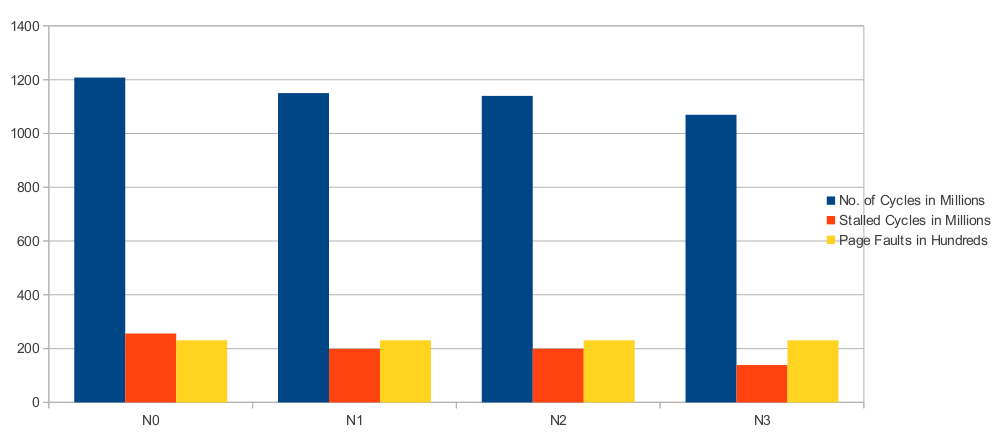
\includegraphics[scale=0.38]{remoteVsLocal.png}
    \caption{Comparison of remote vs local library. N0, N1, N2, N3 are nodes in NUMA machine. Shared library is at N3 }
    \label{fig:remoteVsLocal}
\end{figure}

We measured the total number of CPU cycles consumed, stalled cycles and page faults in each case.
We observed that in the case when our thread was running locally (i.e. on node N3), it consumed minimum number of CPU cycles.
Number of stalled cycles were also minimum when library is placed locally, high number of stalled cycles in remote case indicates
that a lot of CPU cycles were idle due slowdown for data fetch over the interconnect.
We measured page faults to make sure that we are fetching equal number of library pages in all four cases.
As expected, the number of page faults was found to be equal in all four cases.

It can be verified that N0 and N3 being on the opposite corners of diagonal, have the maximum interconnect delays.
The results exhibit a similar pattern, as in, maximum cycles are consumed by node N0 and the least cycles for the local node N3.
The maximum slowdown is for the farthest node and was found to be 12.9\%.
Based upon the interconnect delays, we may expect the execution on remote node along diagonal to perform 2x slower compared to local
execution, which is not the case. This means that CPU caches combined with prefetching, lessen the performance hit that
could otherwise be observed.

\subsubsection{Small vs Big functions in Library}

In our previous experiment, size of each function was found to be approximately 600 bytes. We believed that with smaller size
functions, there will be less spatial locality and we could see an increased impact on the performance. In this case, the number
of functions was increased, but the size of each function was reduced to approximately 140 bytes per function.\\
The generated functions looked like this:

\texttt{ int f_i()\{return i;\} }

These functions were indexed as usual and called sequentially with an offset equal to L3 cache size, same as in previous case.
Other experimental settings were similar to previous section and shared library was also placed on Node3.
The results for this are shown in figure \ref{fig:smallFunc}.

\begin{figure}
    \centering
    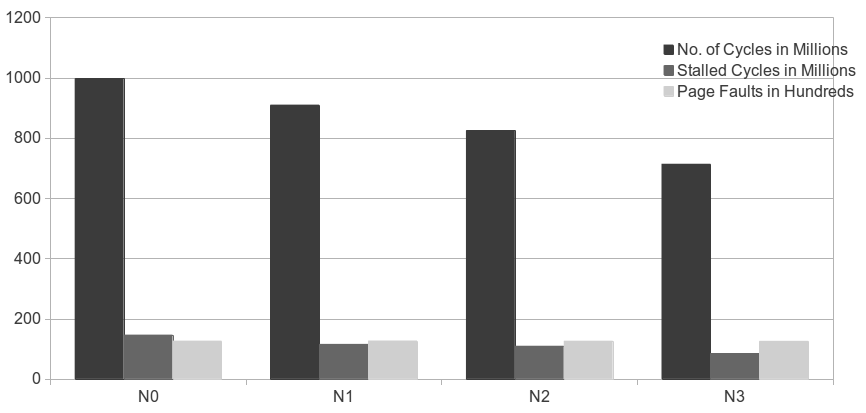
\includegraphics[scale=0.38]{smallFunc.png}
    \caption{Performance with small sized functions. Shared library is at N3 }
    \label{fig:smallFunc}
\end{figure}


It can be seen that the overall execution takes fewer cycles.
This is so because the functions in this case were simpler and compiler could generate better code for them.
The maximum slowdown is again for the farthest node and was found to be close to 39.7\%.
However, it can also be seen that the effect of library being on the remote node is more pronounced here compared to the previous case.
We believe that this is because in the previous case, a prefetched function would exhibit a certain spatial locality of 600 bytes,
which is reduced to 140 bytes in this case.

\subsubsection{Various probability distributions of function calls}

\begin{figure}
    \centering
    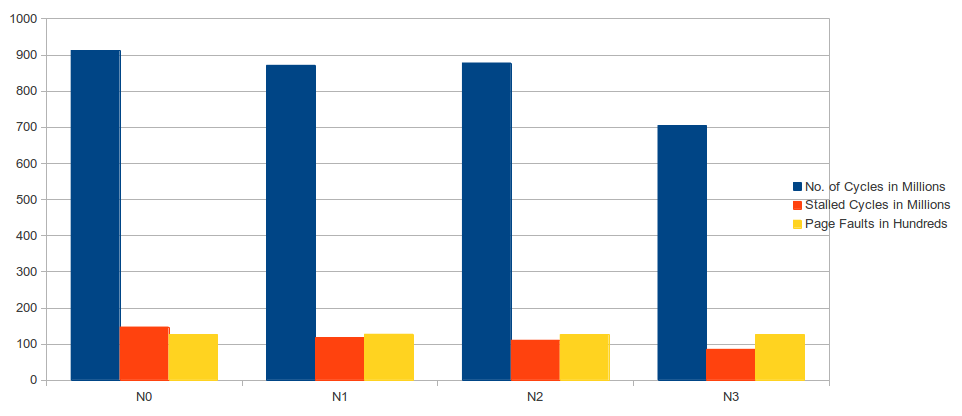
\includegraphics[scale=0.38]{randomDistribution.png}
    \caption{Library functions called in random order by main thread. Shared library is at N3 }
    \label{fig:randomDistribution}
\end{figure}

\begin{figure}
    \centering
    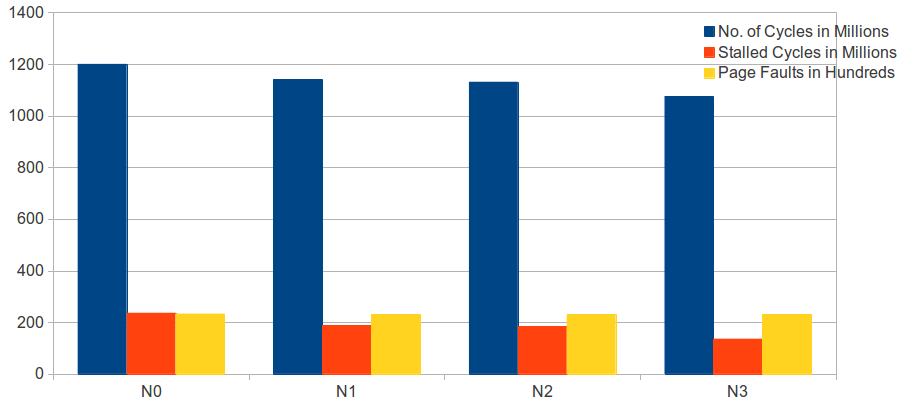
\includegraphics[scale=0.38]{zipfDistribution.png}
    \caption{Library functions called in Zipfian order (with alpha=0.5) by main thread. Shared library is at N3 }
    \label{fig:zipfDistribution}
\end{figure}

Until now we were calling the functions from the shared library in a sequential order.
In real application scenarios it is not necessarily the case that an application is using all the functions 
of a library and that too in sequential order. In an attempt to simulate some real application scenarios,
we tried varying our function calling pattern to random and zipfian distributions.

\textbf{Sequential} - Figure \ref{fig:remoteVsLocal} shows the results for sequential calling pattern\\
\textbf{Random} - Figure \ref{fig:randomDistribution} shows the results for calling library functions in random order.\\
\textbf{Zipf} - Figure \ref{fig:zipfDistribution} shows the results for calling library functions in zipfian order.\\

The maximum slowdown was again for the farthest node in each of the two cases. The performance impact was 12.05\% for
the random distribution, whereas it was 11.57\% for the zipfian order. According to zipfian distribution,
there will be a bunch of functions which will be called more frequently than others. Therefore, the instruction cache
can perform better in this case and consequently the performance impact can be lesser.

\subsubsection{Impact of Library Sizes}

\begin{figure}
    \centering
    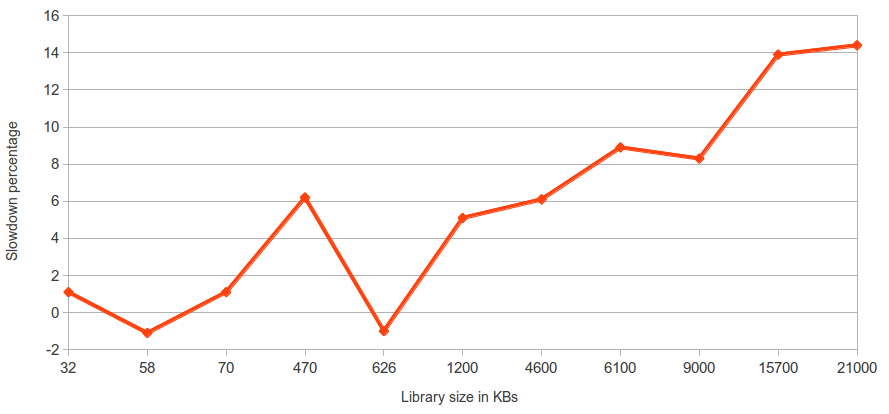
\includegraphics[scale=0.39]{slowdownWithSize.png}
    \caption{Slowdown with increasing library size }
    \label{fig:slowdownWithSize.png}
\end{figure}

In all of the above experiments, the shared library we used had about 60 MB of text-section.
As discussed earlier, most of the modern libraries are lesser than 20 MBs, and very few are of
order of 40 MBs. In this section we will vary the text-section size for the libraries and see 
the impact on system performance.

As the size of text-section is directly proportional to the number of functions, we vary the size by simply 
increasing the number of functions. We generated libraries of sizes varying from 32KB to 21MB, see Figure \ref{fig:slowdownWithSize.png}.
We kept the size of each function same at around 600 Bytes, and increased the number of functions available in each library.
We believe that when the library will be small enough to fit in the cache, there will be very few instruction fetches across the interconnect.
But with the increasing sizes, its likely that there will be more cache misses impacting the performance.

To measure this impact we introduce the following metric:
\begin{dmath}
\label{eqn:cyclesPerCall}
N_{cyclesPerCall} =  N_{totalElapsedCycles} / numFunctionCalls
\end{dmath}

This metric is necessary to compare performance across libraries of two different sizes, as with increased sizes, the number
of page-faults to load the library into memory will also increase.

The main thread calls the library functions in sequential order, each function being called only once.
Setup was very much similar to above experiments, we had our library on one node and main thread was made to run on 
each of the four nodes. For our comparison, we selected the local node (housing the shared library) and farthest node
from this local node, and computed the ratio of their $N_{cyclesPerCall}$ metric as follows:
\begin{dmath}
\label{eqn:slowdown}
R_{slowdown} =  N\_Far_{cyclesPerCall} / N\_Local_{cyclesPerCall}
\end{dmath}

We then plot the values of $R_{slowdown}$ in percentage for different values of library text-section sizes.
The result is shown in Figure \ref{fig:slowdownWithSize.png}.
As expected, we found that when the library is small enough to fit in the cache, not much slowdown is observed.
It has even gone to negative in some cases. But as the size of library increases and the cache misses increase,
we see the the effect of slowdown becomes more pronounced. The slowdown was found to be about 14\% for a library
with 21MB of text section, but later stabilizes around this value.

\begin{figure}
    \centering
    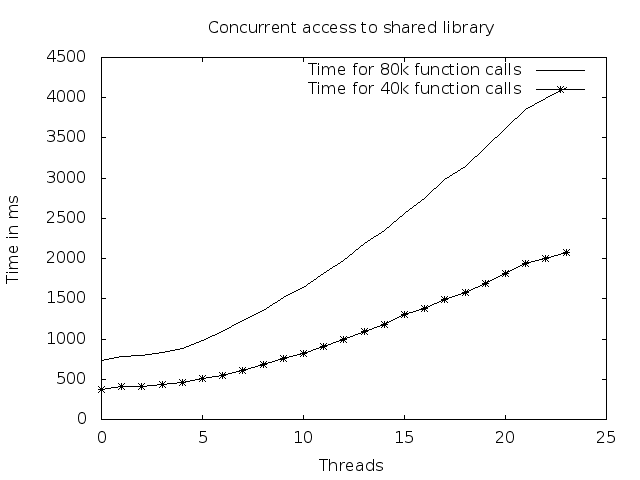
\includegraphics[scale=0.39]{timevsthread_noMem.png}
    \caption{Effect of concurrent access to shared library on increasing the number of threads.}
    \label{fig:timevsthread.png}
\end{figure}

\subsection{Impact of congestion}
Dashti et al. \cite{Dashti:2013:TMH:2490301.2451157} claim that in modern NUMA systems, wire-delays
are not the only source of performance hits, but congestion on interconnect links and in memory 
controllers can also dramatically hurt performance. They propose an algorithm which avoids, traffic
hot-spots to prevent congestion on interconnect and memory controllers.

In case of data, an application may exploit data-level parallelism by splitting the data, such that
each thread mostly works on a distinct data-set. In such a scenario, threads are lightly coupled and
is ideal for parallelism. It also doesn't make much sense for multiple threads to operate on 
same data set in parallel, and therefore it is less likely that traffic hot-spots exist in such a system,
and even if they do exist, can be avoided by careful allocation of data.\\
Such a situation, is however more likely to happen in case of shared libraries, as they can only have
a single copy across the system, making the NUMA node housing the library, a potential traffic hot-spot.

In the previous sections, all our experiments were conducted independently, that is, the shared library
was being accessed only by a single thread. In real application scenarios, multiple threads and processes
can access shared code concurrently. In this section, we present an analysis of what happens when multiple
threads try to access the library concurrently.\\
For this analysis, we are using a smaller more-realistic shared library with 10k functions amounting to about 20M 
of text-section. The shared library was placed on Node 0. The driver function that calls the functions from 
the library can now be executed concurrently by multiple threads.
We don't modify any shared-data, therefore we didn't need any kind of locking or synchronization mechanisms.

Figure \ref{fig:timevsthread.png} shows the plot of time taken for n-threads to execute 40k and 80k function calls from
the library for different values of n. It can be seen that the curve is nearly flat in the beginning, but picks up
later with increase in congestion at the interconnect and/or memory controller.

We also tried various combinations, the results of which are presented below:
\begin{verbatim}
(Library residing on node 0)
Number of running threads : 1
Core 0 : 375.04 ms
Core 3 : 386.42 ms

Number of running threads : 2
Core 0 and  4 : 387.20 (Local memory + shared cache)
Core 1 and  2 : 402.50 (Remote memory + 
                        No shared cache)
Core 3 and  7 : 405.48 (Remote memory +
                        shared cache)

Number of running threads : 3
Core 0, 4 and 8 : 392.31 (All three local +
                          shared cache)
Core 1, 2 and 3 : 411.31 (All remote + 
                          No shared cache)
\end{verbatim}

Based upon these values, it can be inferred that there is a performance overhead, whenever a new thread is
added to the system. Sometimes, this overhead gets reduced when the cores have a shared cache. This is so because
the  threads are accessing the same data, hence the caches will collaborate and not contend. The extra performance
overhead with introduction of new threads can be attributed to congestion on both memory controller and the interconnect.
We believe that the interconnect congestion is less evident with smaller number of threads but becomes more pronounced
when the number of threads increase, which explains the initial flat curve in the graph. At later stages, as each node
can have multiple cores fetching the shared-code from the memory, their caches may be co-operate, resulting in the an
asymptotic curve towards the end.
